\documentclass[french]{article}
 
\usepackage[utf8]{inputenc}
\usepackage[T1]{fontenc}
\usepackage{babel}
\usepackage{graphicx}
\usepackage{amsmath}
\usepackage{caption}
\usepackage{subcaption}

\begin{document}
\section{Dispositif expérimental}
Nous avions à notre dispostion pour effectuer nos mesures une soufferie, un capteur de pression

\begin{figure}
\centering
\begin{subfigure}{.5\textwidth}
  \centering
  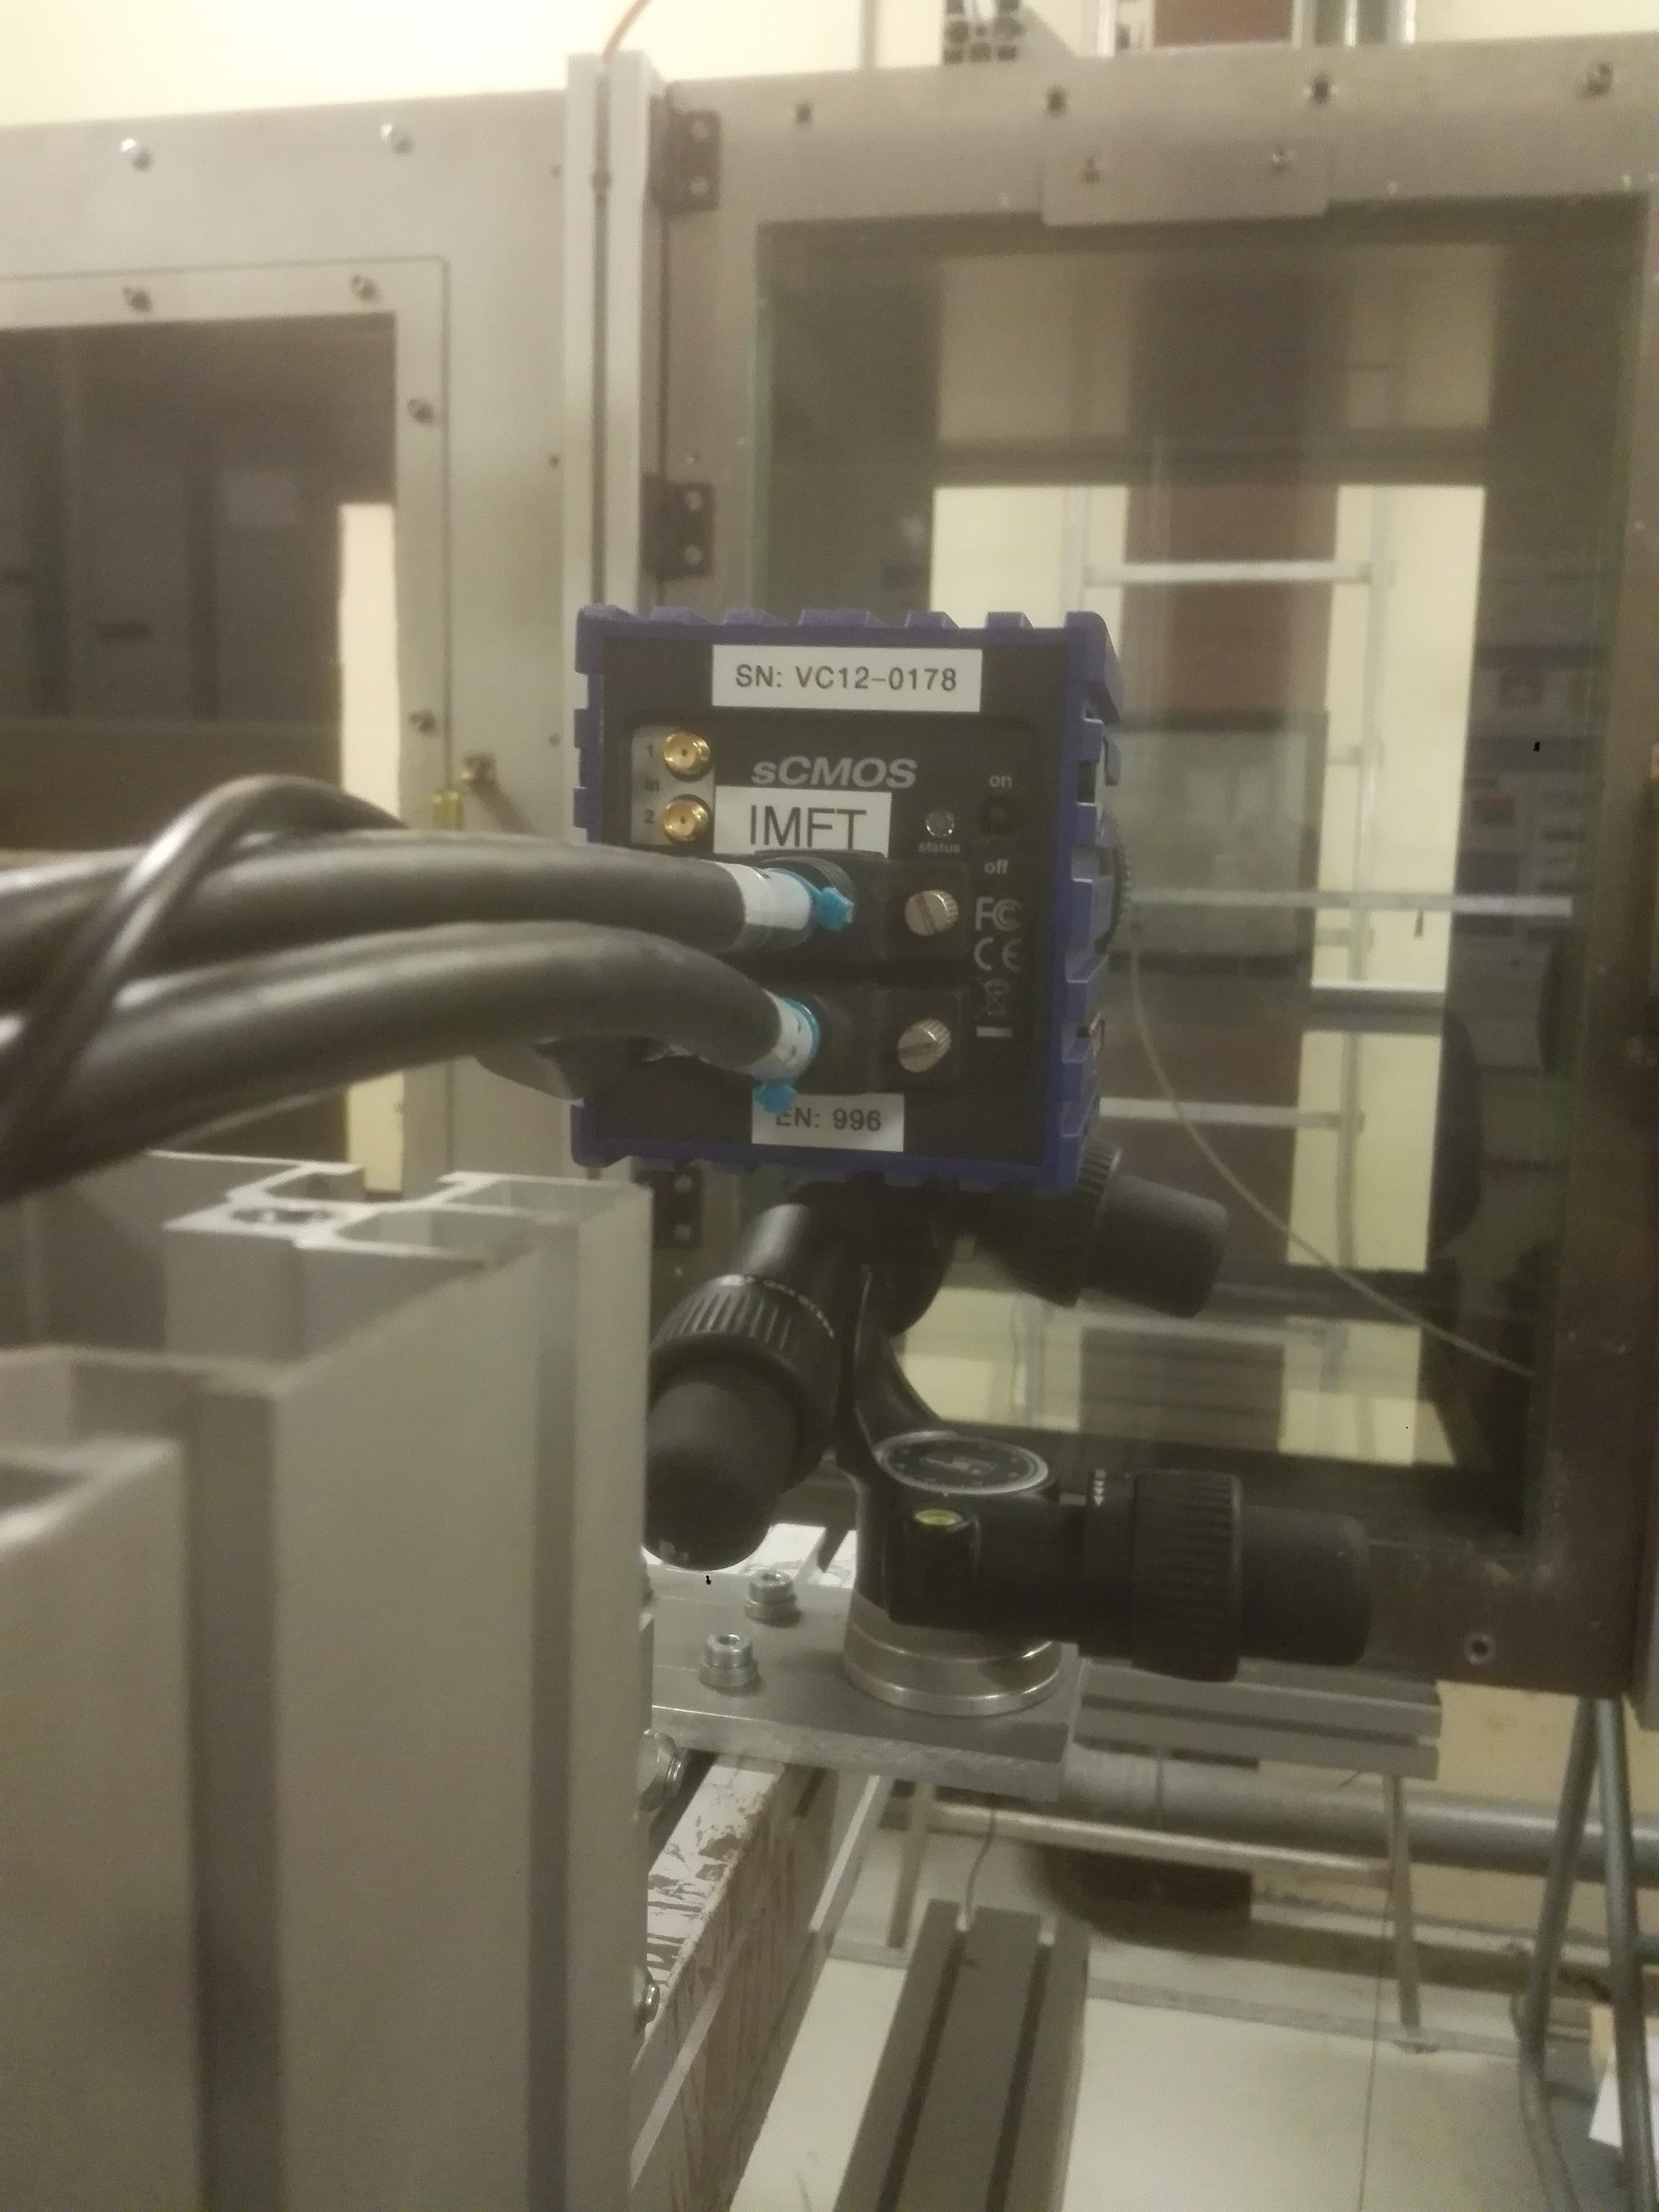
\includegraphics[width=.6\linewidth]{./image/Camera.jpg}
  \caption{Camera}
  \label{fig:sub1}
\end{subfigure}%
\begin{subfigure}{.5\textwidth}
  \centering
  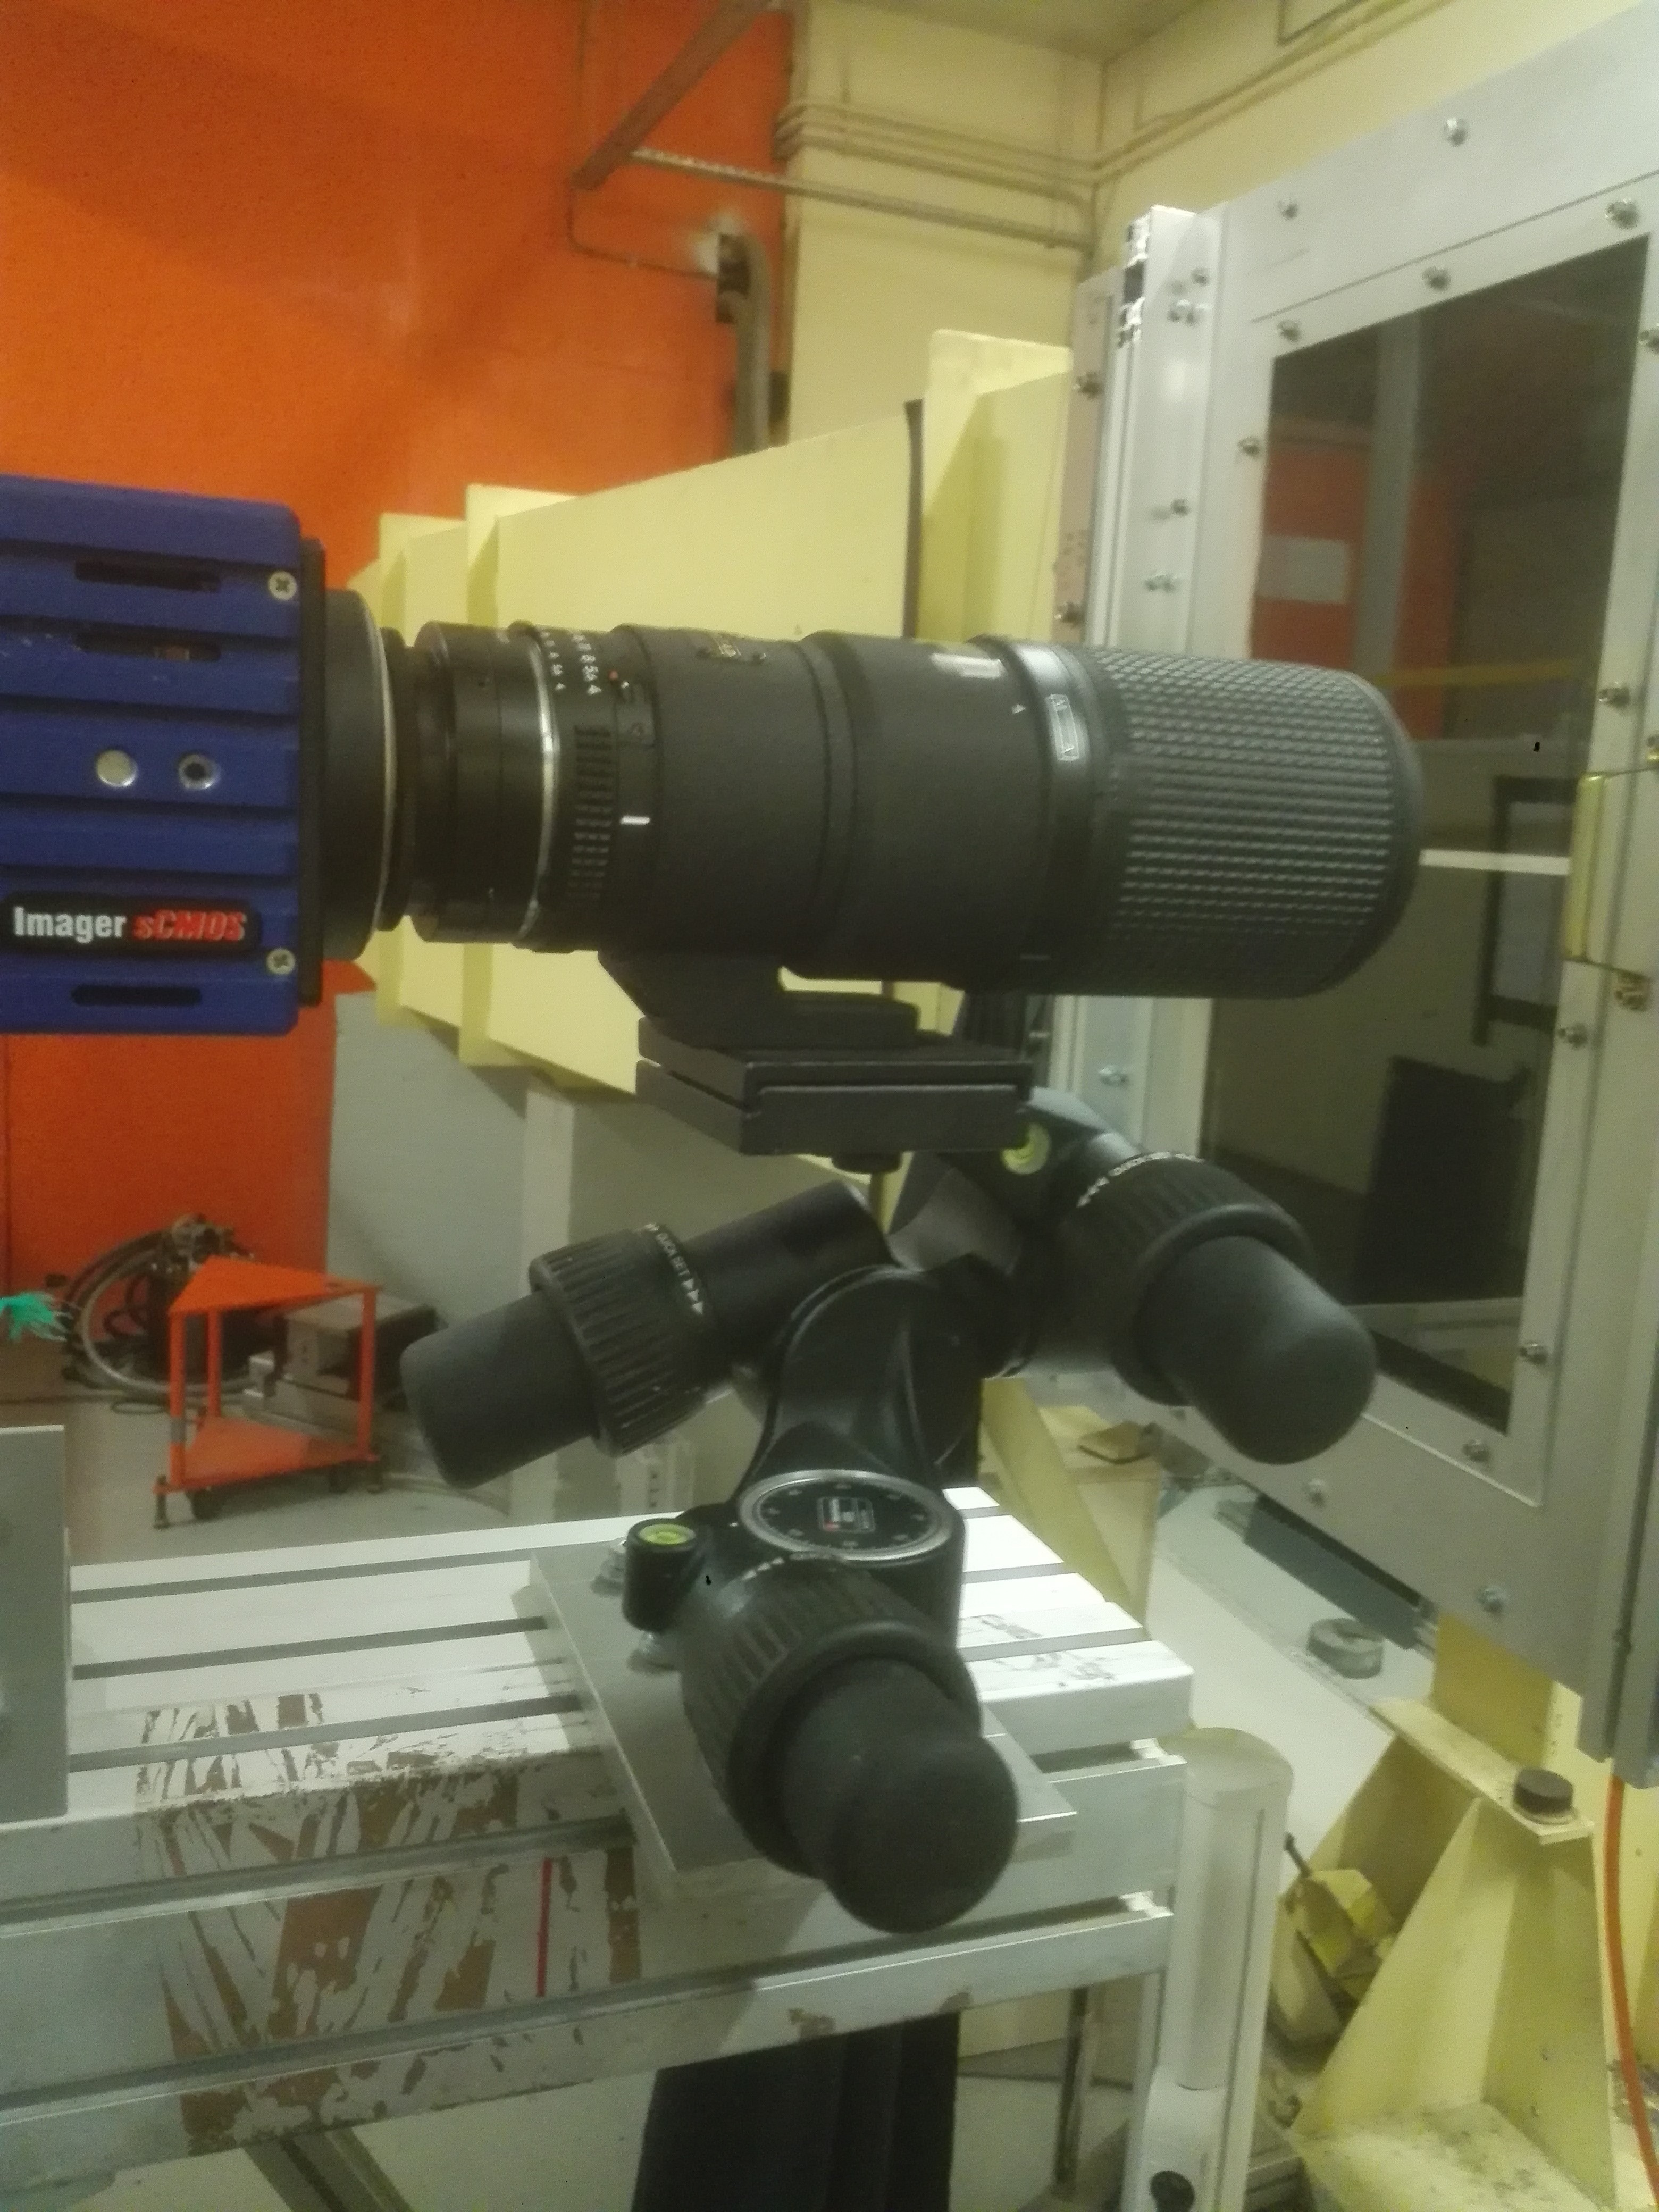
\includegraphics[width=.6\linewidth]{./image/Camera2.jpg}
  \caption{Camera vue de côté}
  \label{fig:Camera}
\end{subfigure}
\caption{Camera}
\label{fig:Camera2}
\end{figure}

\begin{figure}[ht]
\centering
	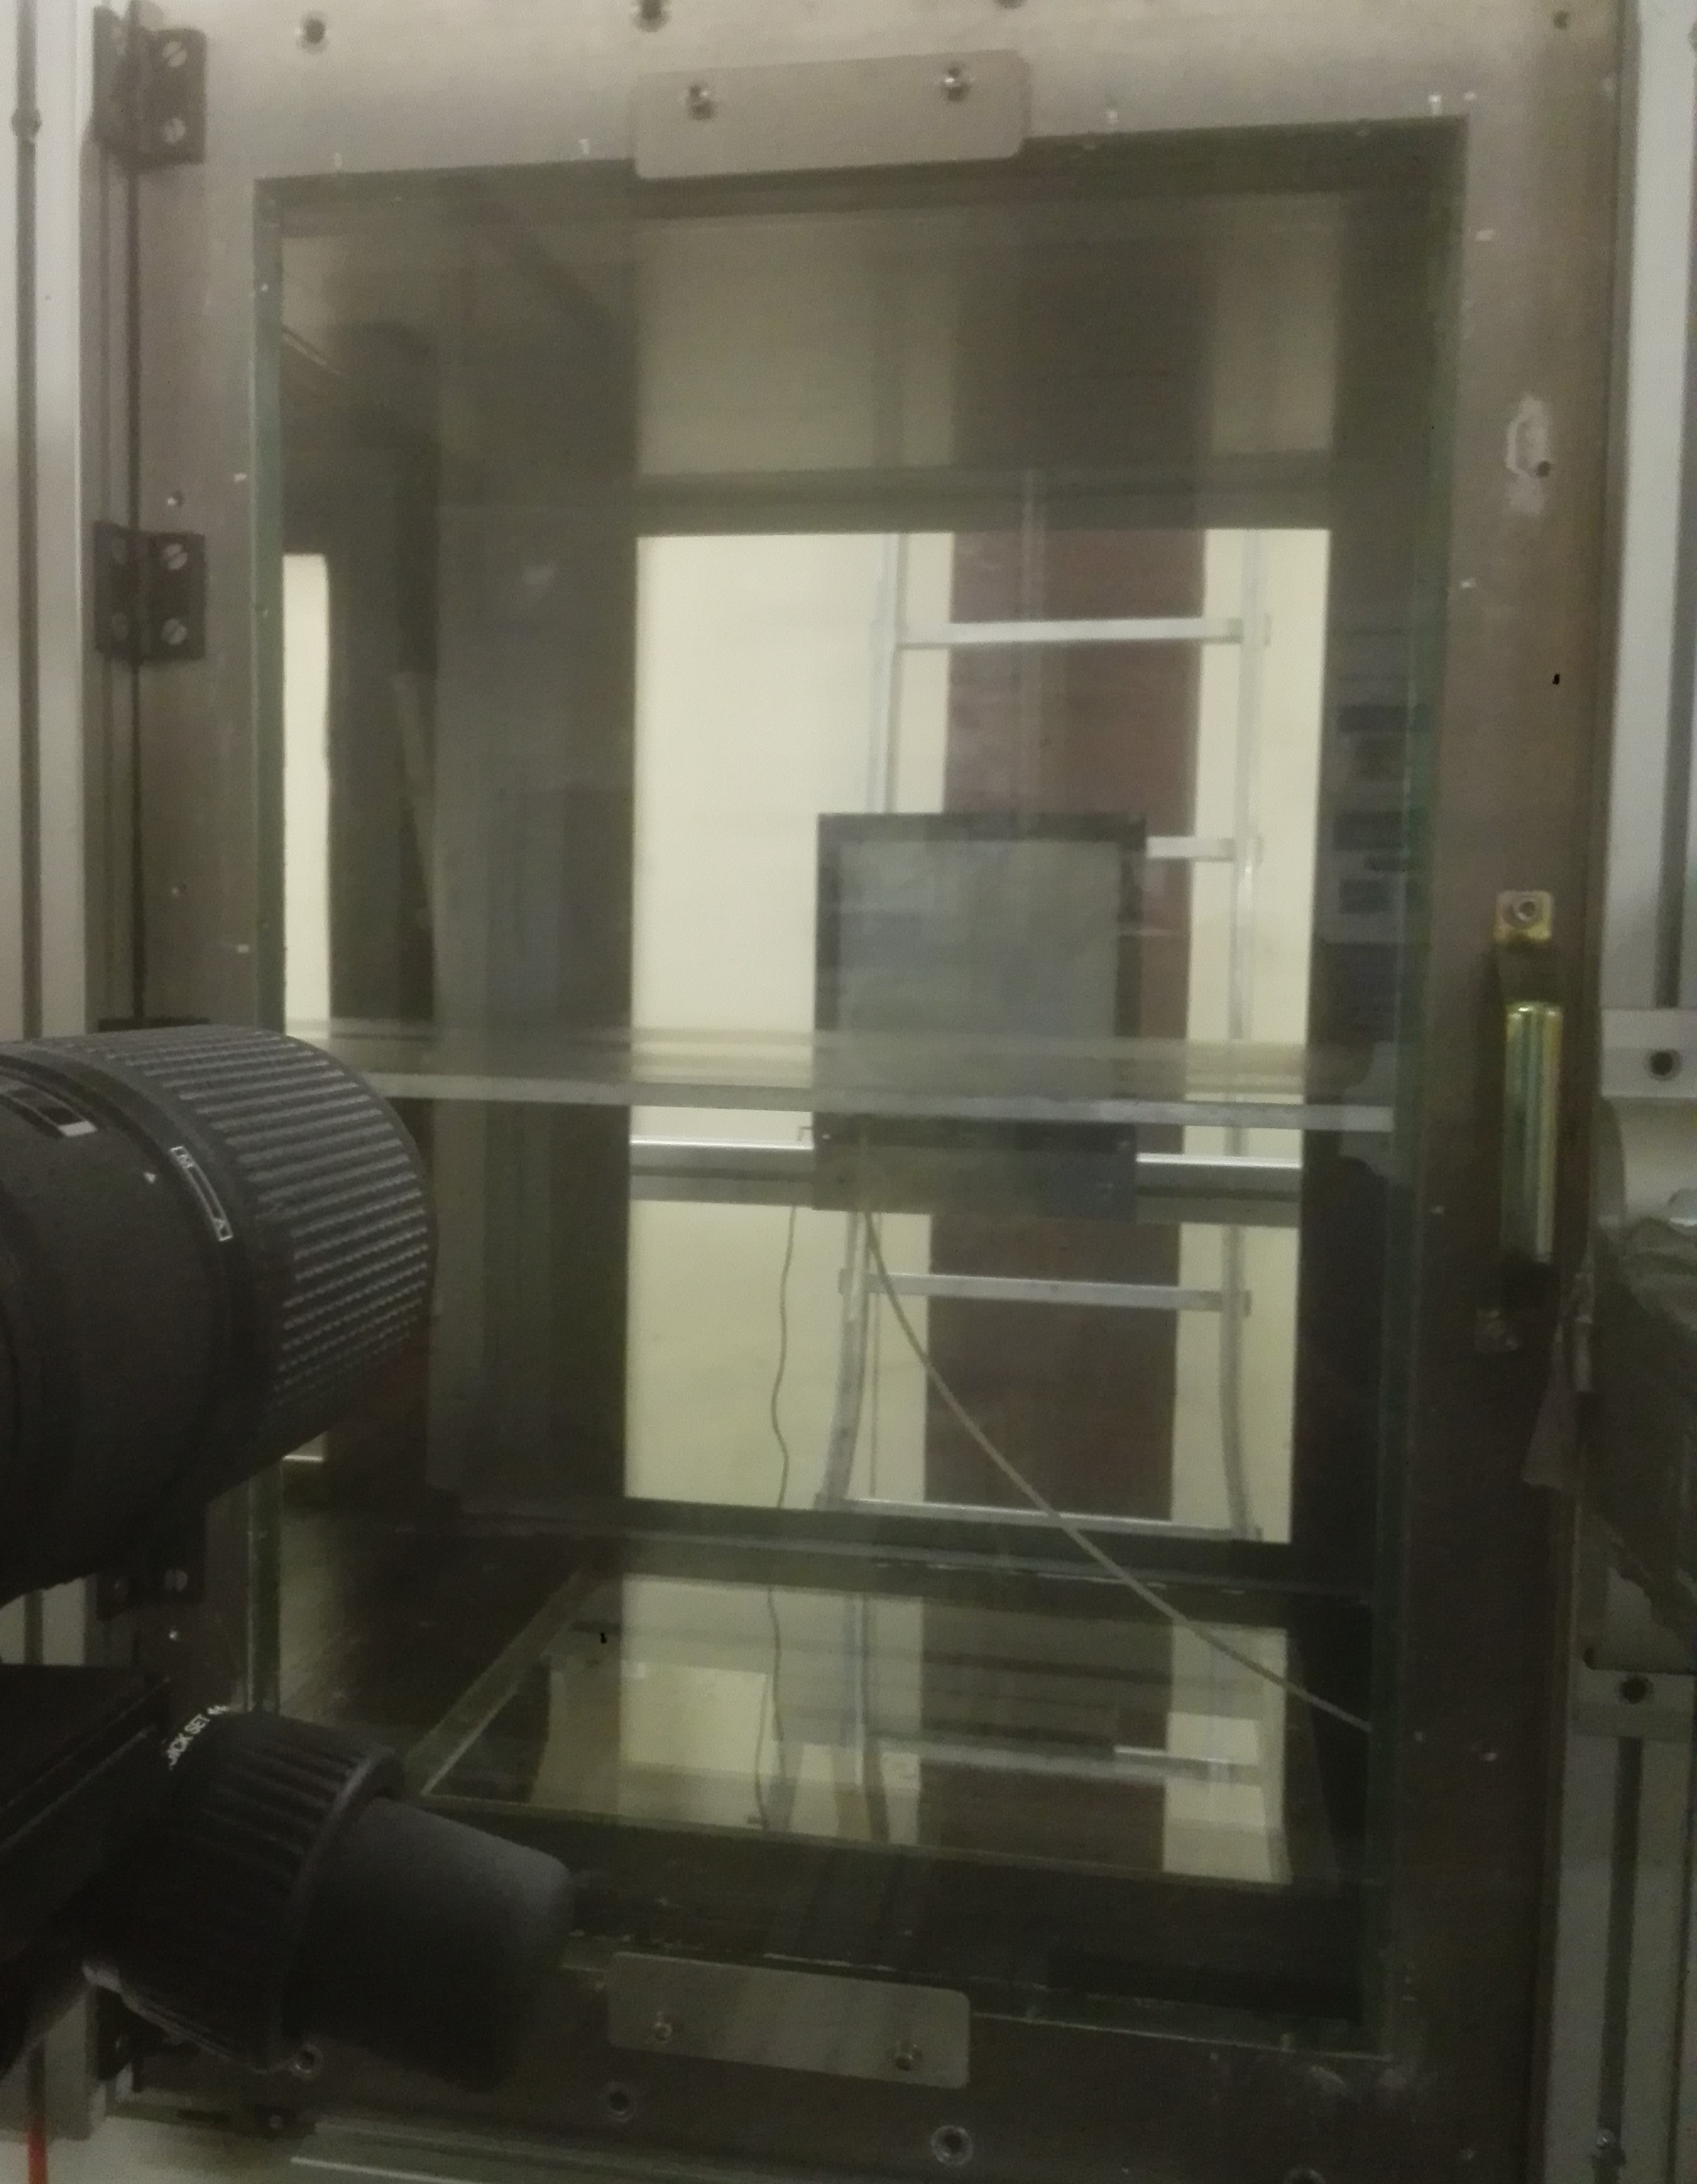
\includegraphics[width = 0.4\linewidth]{./image/Surface.jpg}
	\caption{Plan}
	\label{fig:Plan}
\end{figure}
\begin{figure}[ht]
\centering
	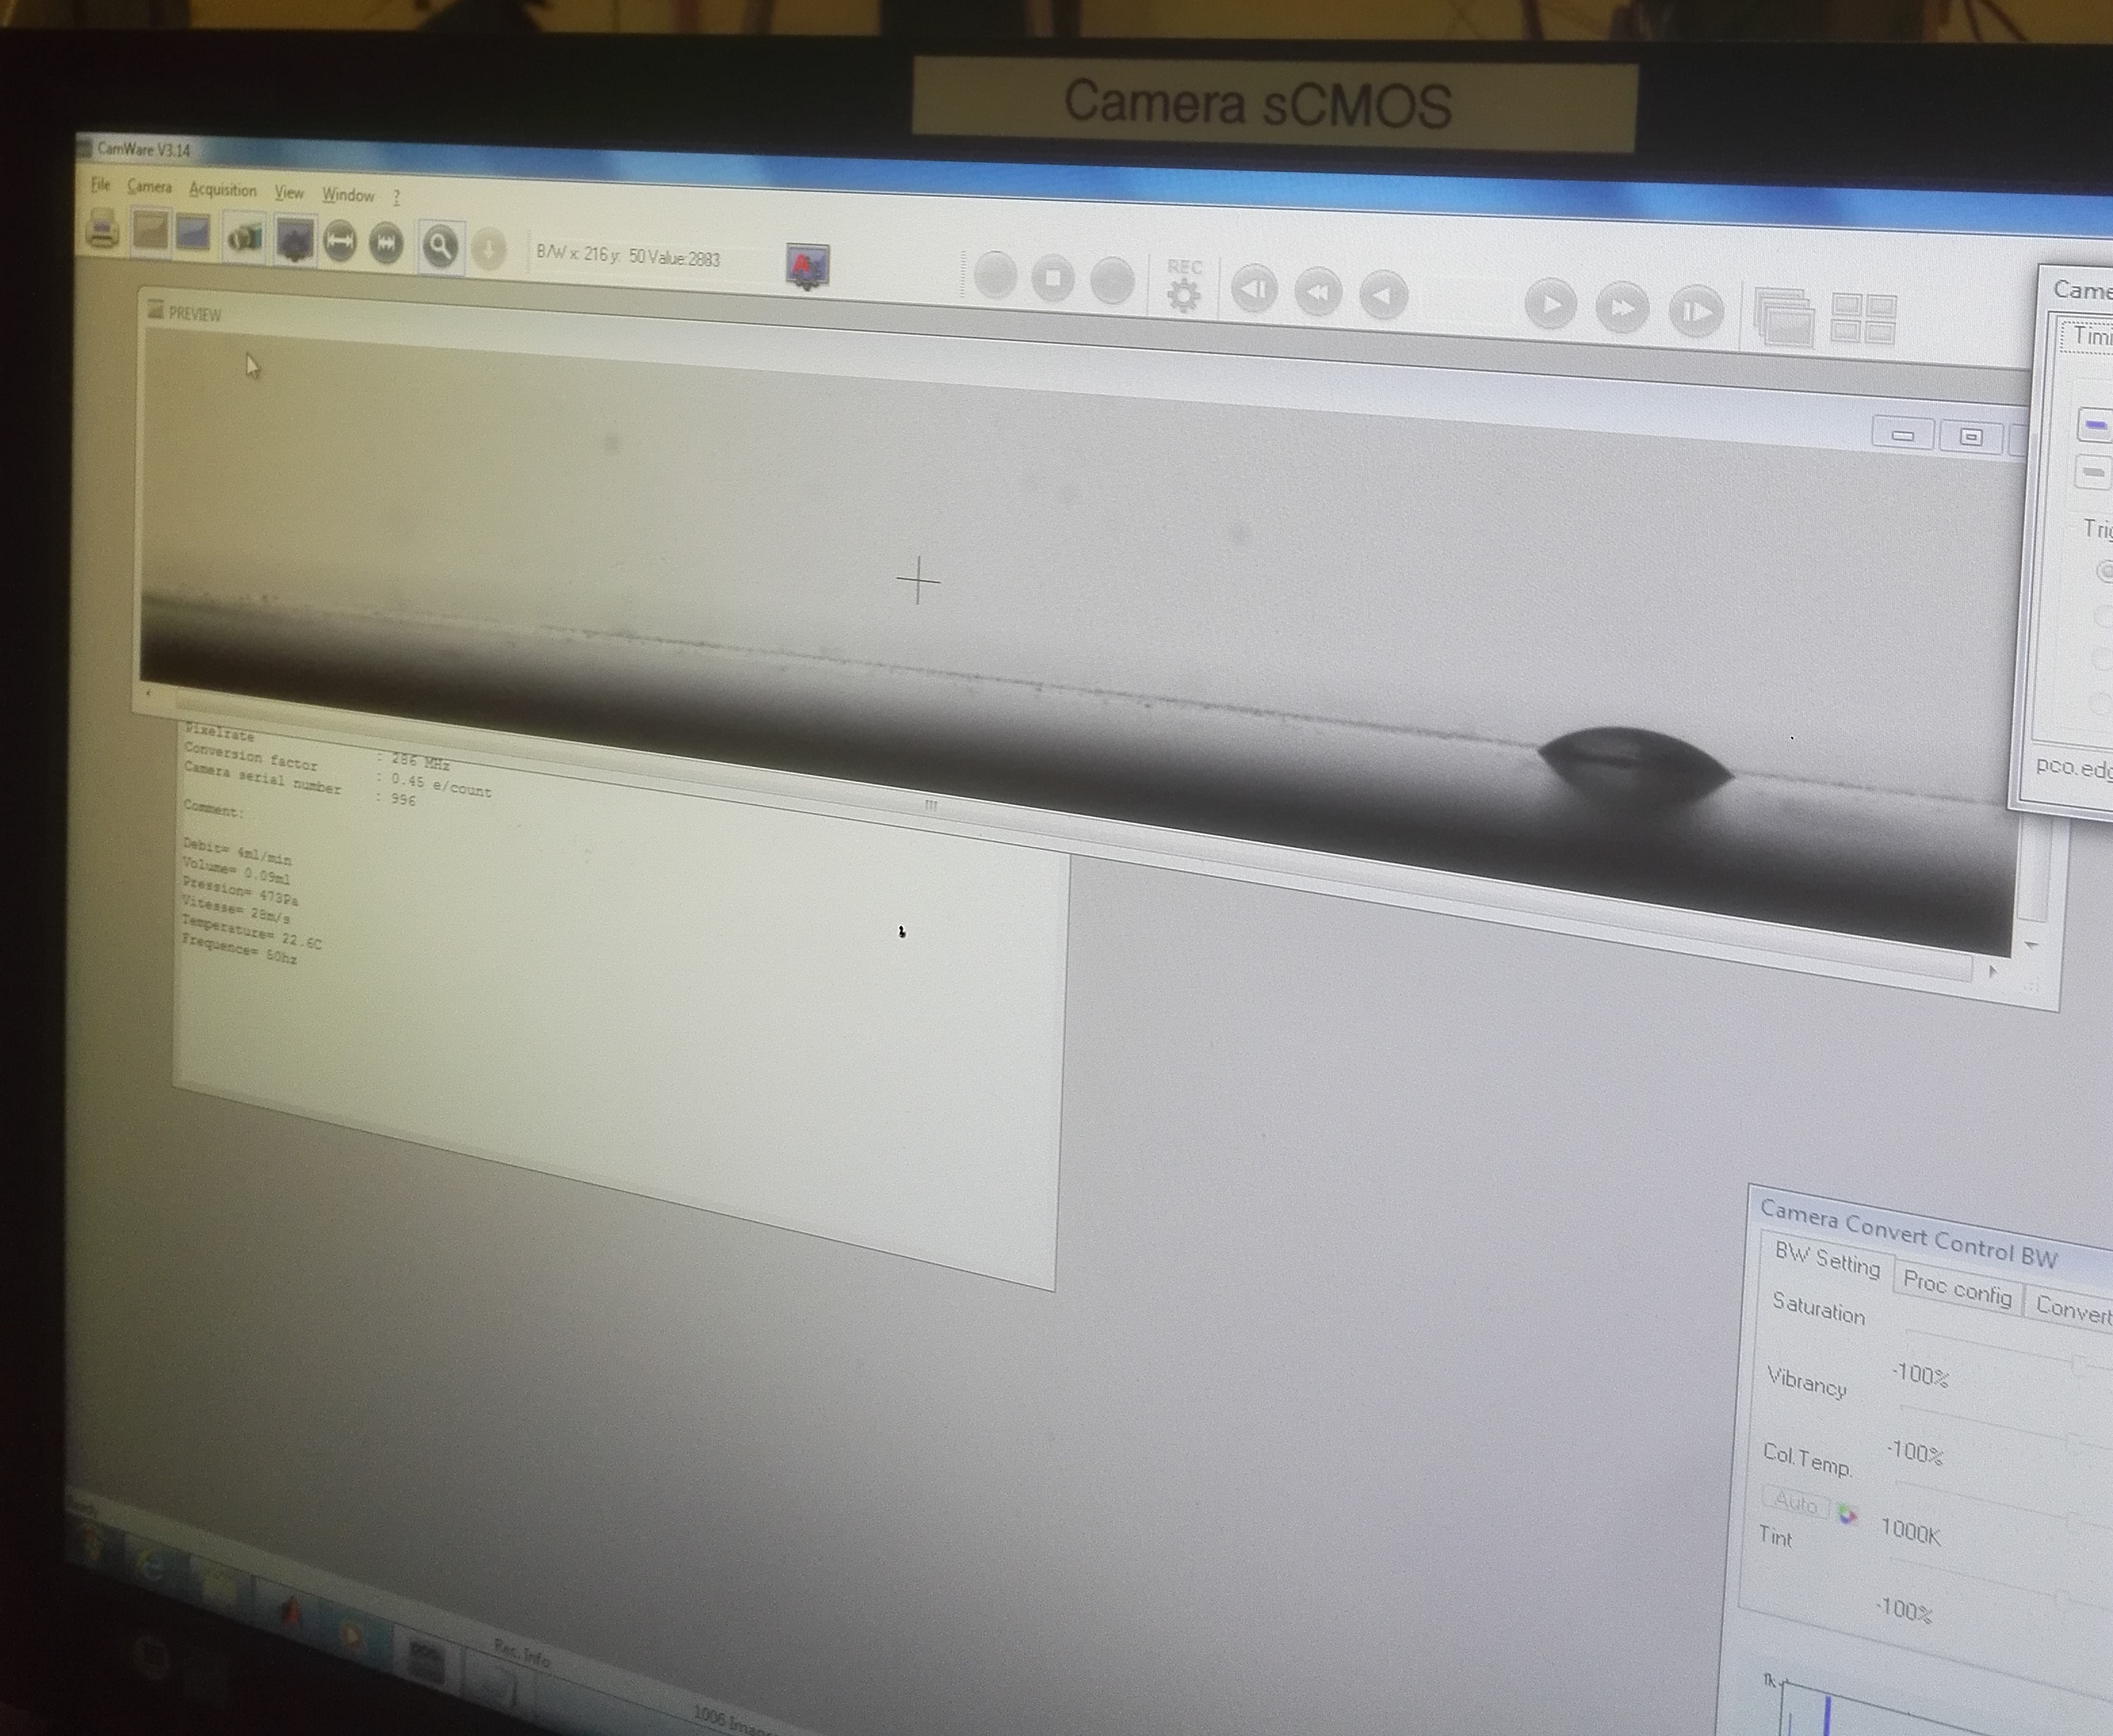
\includegraphics[width = 0.6\linewidth]{./image/Ecran.jpg}
	\caption{Ecran}
	\label{fig:Ecran}
\end{figure}

\section{Anémomètre à fil chaud}
C'est l'anémomètre à fil chaud qui nous a permis de déterminer les profils de la couche limite dans notre.

Le principe de l'anénomètre à fil chaud est de placer un fil chaud dans l'écoulement et de mainternir sa température constante

l'écoulement retirera une énergie au fil chaud et pour maintenir la température constante du fil chaud, on lui fournit une certaine énergie et cette énergie fournie (la tension qu'il a fallu fournir) est liée à la vitesse au niveau du fil chaud.



\begin{figure}[ht]
	\centering
	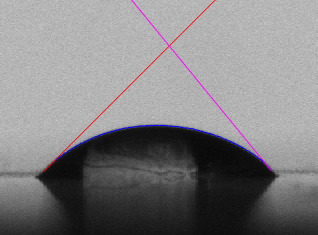
\includegraphics[scale = 0.6]{./image/crop_tvitesse=28_volume=003.png}
	\caption{Goutte d'eau de volume $0.03$ml avec $\theta_{a} = 45^{o}$ et $\theta_{r} = 50.17^{o}$}
\end{figure}

\begin{figure}[ht]
	\centering
	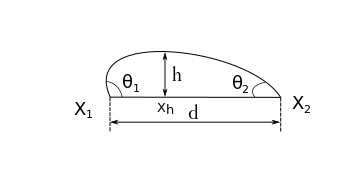
\includegraphics[scale = 1]{./image/rrgou2.png}
	\caption{Paramètres mesurés}
\end{figure}

\end{document}
